\par Pasamos a verificar que se cumple el criterio de Bonello, observando los resultados obtenidos por el programa \quotemarks{\textbf{amroc}}. En la figura \figref{fig:modos_resonancia}, podemos ver que se observa con el requerimiento de que \textbf{la curva resultante debe ser monótona creciente} si consideramos a partir de la octava con frecuencia central de $31.5Hz$, el motivo para descartar las de menor frecuencia, en donde el criterio no se cumple, es que ocurre a frecuencias muy bajas del rango audible.


\begin{figure}[H]
	\centering
	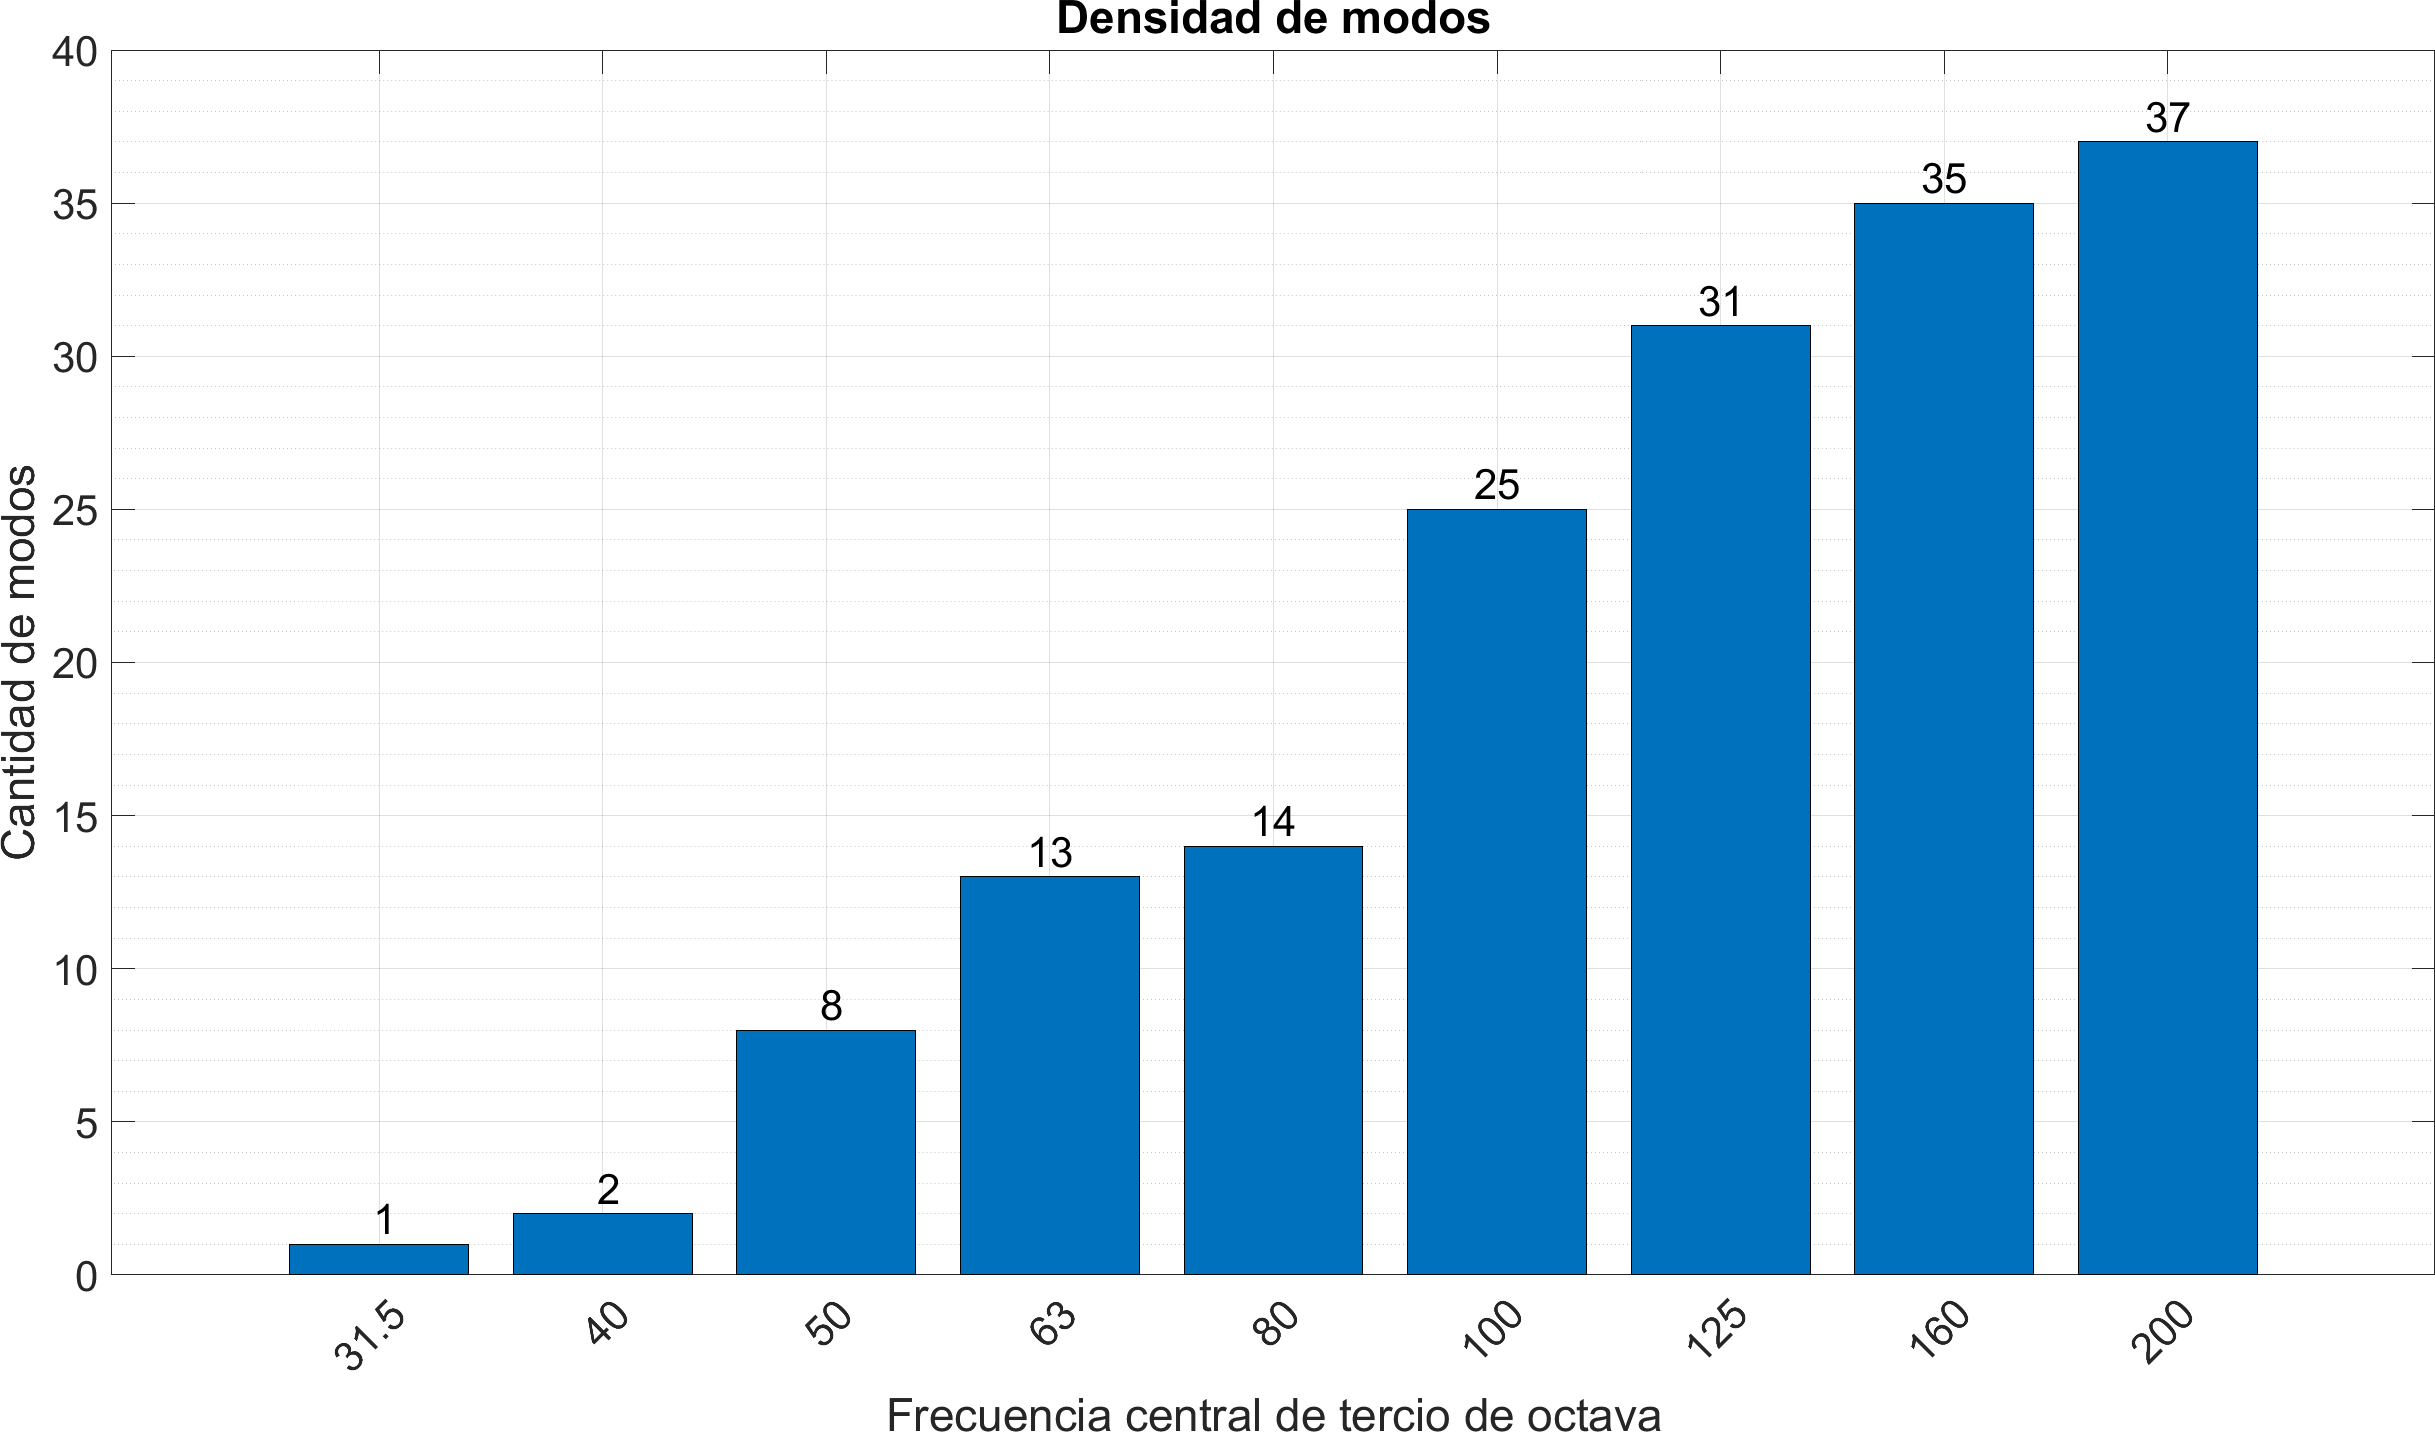
\includegraphics[width=1\textwidth]{./img/modos_resonancia.png}
	\caption{Densidad de nodos por banda de tercio de octava}
	\label{fig:modos_resonancia}
\end{figure}

\newpage

\begin{table}[H]
\setlength\arrayrulewidth{1pt}
\arrayrulecolor{TABLEColor}
    \centering
    \begin{tabular}{|c|c|c|c|c|}
    \hline
N° It. & Frequencia & Nota & $p$,$q$,$r$ & Dirección \\
\hline \hline
5&33.64 Hz&C1&2-1-0&tan\\
6&37.01 Hz&D1&3-0-0&ax\\
7&43.51 Hz&F1&3-1-0&tan\\
8&45.73 Hz&F1\#&0-2-0&ax\\
9&47.37 Hz&F1\#&1-2-0&tan\\
10&49.35 Hz&G1&4-0-0&ax\\
11&50.44 Hz&G1\#&0-0-1&ax\\
12&51.93 Hz&G1\#&1-0-1&tan\\
13&51.97 Hz&G1\#&2-2-0&tan\\
14&54.39 Hz&A1&4-1-0&tan\\
15&55.38 Hz&A1&0-1-1&tan\\
16&56.15 Hz&A1&2-0-1&tan\\
17&56.74 Hz&A1\#&1-1-1&obl\\
18&58.84 Hz&A1\#&3-2-0&tan\\
19&60.63 Hz&B1&2-1-1&obl\\
20&61.69 Hz&B1&5-0-0&ax\\
21&62.56 Hz&B1&3-0-1&tan\\
22&65.79 Hz&C2&5-1-0&tan\\
23&66.61 Hz&C2&3-1-1&obl\\
24&67.28 Hz&C2&4-2-0&tan\\
25&68.09 Hz&C2\#&0-2-1&tan\\
26&68.6 Hz&C2\#&0-3-0&ax\\
27&69.2 Hz&C2\#&1-2-1&obl\\
28&69.7 Hz&C2\#&1-3-0&tan\\
29&70.57 Hz&C2\#&4-0-1&tan\\
30&72.42 Hz&D2&2-2-1&obl\\
31&72.9 Hz&D2&2-3-0&tan\\
32&74.03 Hz&D2&6-0-0&axv\\
33&74.18 Hz&D2&4-1-1&obl\\
34&76.79 Hz&D2\#&5-2-0&tan\\
35&77.48 Hz&D2\#&6-1-0&tan\\
36&77.5 Hz&D2\#&3-2-1&obl\\
37&77.95 Hz&D2\#&3-3-0&tan\\
38&79.69 Hz&D2\#&5-0-1&tan\\
39&82.9 Hz&E2&5-1-1&obl\\
40&84.09 Hz&E2&4-2-1&obl\\
41&84.51 Hz&E2&4-3-0&tan\\
42&85.15 Hz&F2&0-3-1&tan\\
43&86.04 Hz&F2&1-3-1&obl\\
44&86.37 Hz&F2&7-0-0&ax\\
45&87.02 Hz&F2&6-2-0&tan\\
46&88.65 Hz&F2&2-3-1&obl\\
47&89.34 Hz&F2&7-1-0&tan\\
48&89.58 Hz&F2&6-0-1&tan\\
49&91.47 Hz&F2\#&0-4-0&ax\\
\hline
    \end{tabular}
    \quad
    \begin{tabular}{|c|c|c|c|c|c|}
    \hline
N° It. & Frequencia & Nota & $p$,$q$,$r$ & Dirección \\
\hline \hline
50&91.88 Hz&F2\#&5-2-1&obl\\
51&92.26 Hz&F2\#&5-3-0&tan\\
52&92.3 Hz&F2\#&1-4-0&tan\\
53&92.45 Hz&F2\#&6-1-1&obl\\
54&92.85 Hz&F2\#&3-3-1&obl\\
55&94.74 Hz&F2\#&2-4-0&tan\\
56&97.73 Hz&G2&7-2-0&tan\\
57&98.42 Hz&G2&4-3-1&obl\\
58&98.67 Hz&G2&3-4-0&tan\\
59&98.71 Hz&G2&8-0-0&ax\\
60&100.02 Hz&G2&7-0-1&tan\\
61&100.58 Hz&G2&6-2-1&obl\\
62&100.88 Hz&G2\#&0-0-2&ax\\
63&100.93 Hz&G2\#&6-3-0&tan\\
64&101.32 Hz&G2\#&8-1-0&tan\\
65&101.63 Hz&G2\#&1-0-2&tan\\
66&102.6 Hz&G2\#&7-1-1&obl\\
67&103.44 Hz&G2\#&0-1-2&tan\\
68&103.86 Hz&G2\#&2-0-2&tan\\
69&103.93 Hz&G2\#&4-4-0&tan\\
70&104.17 Hz&G2\#&1-1-2&obl\\
71&104.45 Hz&G2\#&0-4-1&tan\\
72&105.15 Hz&G2\#&5-3-1&obl\\
73&105.18 Hz&G2\#&1-4-1&obl\\
74&106.34 Hz&G2\#&2-1-2&obl\\
75&107.33 Hz&A2&2-4-1&obl\\
76&107.46 Hz&A2&3-0-2&tan\\
77&108.79 Hz&A2&8-2-0&tan\\
78&109.86 Hz&A2&3-1-2&obl\\
79&109.98 Hz&A2&7-2-1&obl\\
80&110.3 Hz&A2&7-3-0&tan\\
81&110.33 Hz&A2&5-4-0&tan\\
82&110.76 Hz&A2&0-2-2&tan\\
83&110.82 Hz&A2&3-4-1&obl\\
84&110.85 Hz&A2&8-0-1&tan\\
85&111.04 Hz&A2&9-0-0&ax\\
86&111.45 Hz&A2&1-2-2&obl\\
87&112.31 Hz&A2&4-0-2&tan\\
88&112.83 Hz&A2&6-3-1&obl\\
89&113.18 Hz&A2&8-1-1&obl\\
90&113.37 Hz&A2\#&9-1-0&tan\\
91&113.48 Hz&A2\#&2-2-2&obl\\
92&114.33 Hz&A2\#&0-5-0&ax\\
93&114.61 Hz&A2\#&4-1-2&obl\\
94&115 Hz&A2\#&1-5-0&tan\\
\hline
    \end{tabular}
    \caption{Datos obtenidos por el programa}
    \label{tab:datos_obtenidos_programa}
\end{table}


\newpage

\par Luego en el cuadro \tableref{tab:datos_obtenidos_programa}, verificamos el criterio el cuál \textbf{no deben existir modos dobles}, para las frecuencias obtenidas cuando la densidad de modos es menor a cinco.\\


\par Previamente, mencionamos que los modos son calculados hasta alcanzar la \textit{frecuencia de Schroeder}. Dicha frecuencia se calcula según la ecuación \eqref{eq::freq_schroeder}.

\begin{equation}
    \boxed{f_s = 1893 \cdot \sqrt{\frac{TR}{V}}}
    \label{eq::freq_schroeder}
\end{equation}

%\par Según los datos provistos obtenidos por el programa, el mismo considera la norma \textbf{DIN 18041} pensada para discurso en sala, que establece un tiempo de reverberación $RT60 = 0.8s$ por lo tanto, según el software \textbf{amroc}, se obtiene que la frecuencia de Schroeder es $95Hz$. Utilizando los valores de la sala diseñada, utilizando la ecuación \eqref{eq::freq_schroeder} obtenemos que la frecuencia de Schroeder es 





\par La frecuencia de Schroeder está en la zona de transición de la respuesta en frecuencia de un recinto que separa la región de baja frecuencia, dominada por modos separados, y la región de frecuencias dominada por una gran superposición de modos, hasta percibirse como un continuo.\\

\par También mediante los resultados del programa se obtiene la distancia crítica cuyo valor es igual a $1.2m$, cuyo valor calcularemos nuevamente para analizar los materiales que se incluirán en la sala para la \textit{ETAPA 2}.\\

\par Finalmente, dados las medidas de la sala, se realizó un bosquejo de como esta será construida. Utilizando el software \textit{Home By Me} se presenta en la figura~\figref{fig:vista_sup_sala} una vista superior de la sala a construir, y en la figura \figref{fig:vista_3D_sala}~una vista 3D.

\begin{figure}[H]
	\centering
	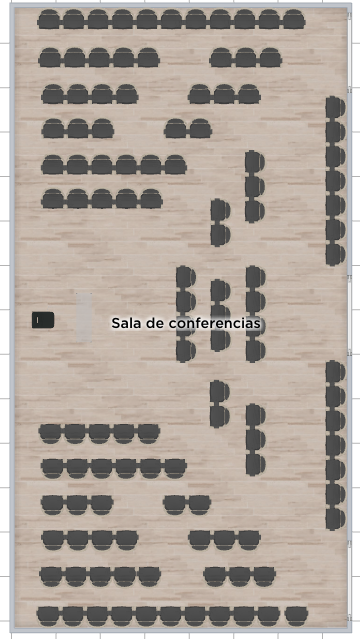
\includegraphics[width=0.6\textwidth]{./img/sala.png}
	\caption{Vista superior de la sala de conferencias}
	\label{fig:vista_sup_sala}
\end{figure}


\begin{figure}[H]
	\centering
	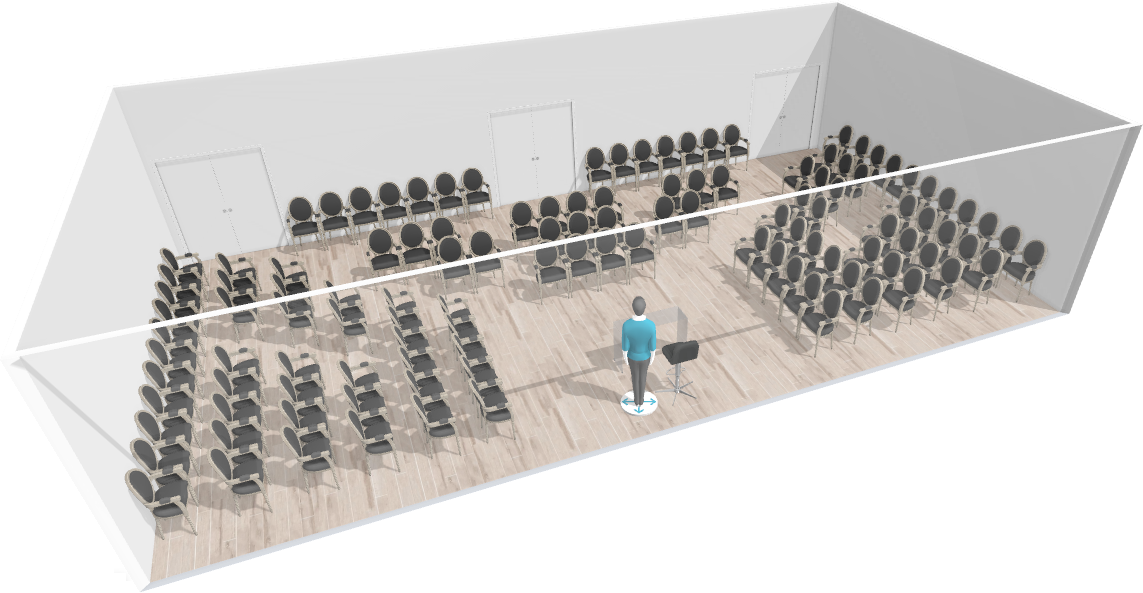
\includegraphics[width=1\textwidth]{./img/sala3D.png}
	\caption{Vista 3D de la sala de conferencias}
	\label{fig:vista_3D_sala}
\end{figure}


\par En el cuadro se presentan los datos de las distancias entre butacas:

\begin{table}[H]
\setlength\arrayrulewidth{1pt}
\arrayrulecolor{TABLEColor}
    \centering
    \begin{tabular}{|c|c|} \hline
        Distancia horizontal entre butacas & 0 cm  \\ \hline
        Distancia posterior entre butacas  & 45 cm  \\ \hline
        Cantidad de butacas & 120 \\ \hline
    \end{tabular}
    \caption{Datos de disposición de butacas}
    \label{tab:my_label}
\end{table}

\par Para el diseño de la sala se consideró mantener equidistante al orador, respecto al público. Se presentan pasillos entre las filas de las butacas para el fácil acceso a los asientos, tres puertas dobles para reducir el tiempo de desalojo en caso de emergencia. Se consideraron filas de butacas contra las paredes con pasillos amplios en su frente, destinadas a posibles tareas periodísticas. La sala posee capacidad para 120 personas. Se adjunta (Figura \figref{fig:plano}) a continuación el boceto de un plano estimado de la sala propuesta, este podrá modificarse en la implementación de fonoabsorbentes. 


\begin{figure}[H]
	\centering
	\includegraphics[width=0.7\textwidth]{./img/sala_medidas.jpg}
	\caption{Boceto del plano de la Sala de Conferencias.}
	\label{fig:plano}
\end{figure}
